\documentclass[journal]{IEEEtran}
\usepackage{amsmath,amssymb,amsfonts}
\usepackage{graphicx}
\usepackage{booktabs}
\usepackage{siunitx}
\usepackage[hidelinks]{hyperref}
\makeatletter
\setlength{\@fptop}{0pt}
\setlength{\@dblfptop}{0pt}
\makeatother
\hypersetup{
  pdftitle={Supplementary Material: Complementary-Filtered Residual World Models for Receding-Horizon Control of Nonlinear Systems},
  pdfauthor={},pdfsubject={},pdfkeywords={}
}
\newcommand{\method}{CFR-WM}
\newcommand{\vect}[1]{\mathbf{#1}}
% Generated only from locked results/confirmatory_analysis artifacts.
\newcommand{\PrimaryBaseline}{PGNN-style}
\newcommand{\PrimaryDifference}{-0.0098}
\newcommand{\PrimaryCILow}{-0.0121}
\newcommand{\PrimaryCIHigh}{-0.0075}
\newcommand{\PrimaryImprovement}{8.97}
\newcommand{\PrimaryRelativeCILow}{6.88}
\newcommand{\PrimaryRelativeCIHigh}{10.95}
\newcommand{\PrimaryPValue}{0.00391}
\newcommand{\PrimaryDecision}{supported}
\newcommand{\PrimaryInterpretation}{supports the prespecified practical-gain claim}
\newcommand{\RobustnessDecision}{not supported}
\newcommand{\RobustnessInterpretation}{does not support the gated robustness claim}
\newcommand{\CorruptImprovement}{12.05}
\newcommand{\CorruptRelativeCILow}{10.51}
\newcommand{\CorruptRelativeCIHigh}{13.49}
\newcommand{\CorruptPValue}{0.00391}
\newcommand{\CleanImprovement}{-13.08}
\newcommand{\CleanRelativeCILow}{-20.60}
\newcommand{\CleanRelativeCIHigh}{-5.67}
\newcommand{\CleanPValue}{0.95703}
\newcommand{\CFRNRMSE}{0.0998}
\newcommand{\PGNNNRMSE}{0.1096}
\newcommand{\BestMethod}{CFR-WM}
\newcommand{\BestNRMSE}{0.0998}
\newcommand{\BestGain}{0.50}
\newcommand{\OneStepImprovement}{59.38}
\newcommand{\OneStepRelativeCILow}{48.88}
\newcommand{\OneStepRelativeCIHigh}{68.88}
\newcommand{\OneStepHolmP}{0.03906}
\newcommand{\CellsWorseTen}{3}
\newcommand{\CartpoleCleanChange}{+47.3}
\newcommand{\VanDerPolCleanChange}{+19.4}
\newcommand{\DuffingCleanChange}{+24.4}
\newcommand{\IDCorruptFavoredCount}{5}
\newcommand{\IDCorruptCellCount}{5}
\newcommand{\IDCorruptLeastChange}{-13.3}
\newcommand{\IDCorruptMostChange}{-34.8}
\newcommand{\AllMetricsFinite}{yes}
\newcommand{\UniqueDataHashes}{40}
\newcommand{\ConfirmatoryRuns}{440}
\newcommand{\ConfirmatoryTrajectories}{126{,}720}

\newcommand{\PosthocBestResidualScale}{0}
\newcommand{\ProjectionMissingEntries}{5404}
\newcommand{\ProjectionChangedFraction}{75.4}
\newcommand{\ProjectionMeanChange}{0.0328}
\newcommand{\ProjectionPChange}{0.1374}
\newcommand{\ProjectionMaxChange}{0.3848}
\newcommand{\CFRLatencyMean}{0.416}
\newcommand{\CFRLatencySD}{0.015}
\newcommand{\ResidualReconstructionDifference}{0.00e+00}
\newcommand{\ExternalMeanReconstructionDifference}{0.00e+00}

% Generated from verified saved external forecasts.
\newcommand{\ExternalTestFlights}{3}
\newcommand{\ExternalFinalSeeds}{5}
\newcommand{\ExternalLearnedParameters}{47000}
\newcommand{\ExternalForecastWindows}{387}
\newcommand{\ExternalCFRCombinedShortNRMSEMean}{0.401}
\newcommand{\ExternalCFRCombinedShortNRMSESD}{0.011}
\newcommand{\ExternalCFRCombinedShortPositionMean}{0.058}
\newcommand{\ExternalCFRCombinedShortPositionSD}{0.002}
\newcommand{\ExternalCFRCombinedShortVelocityMean}{0.133}
\newcommand{\ExternalCFRCombinedShortVelocitySD}{0.002}
\newcommand{\ExternalCFRCombinedLongNRMSEMean}{0.540}
\newcommand{\ExternalCFRCombinedLongNRMSESD}{0.014}
\newcommand{\ExternalCFRCombinedLongPositionMean}{0.094}
\newcommand{\ExternalCFRCombinedLongPositionSD}{0.004}
\newcommand{\ExternalCFRCombinedLongVelocityMean}{0.267}
\newcommand{\ExternalCFRCombinedLongVelocitySD}{0.014}
\newcommand{\ExternalCFRMissingShortNRMSEMean}{0.397}
\newcommand{\ExternalCFRMissingShortNRMSESD}{0.011}
\newcommand{\ExternalCFRMissingShortPositionMean}{0.038}
\newcommand{\ExternalCFRMissingShortPositionSD}{0.002}
\newcommand{\ExternalCFRMissingShortVelocityMean}{0.116}
\newcommand{\ExternalCFRMissingShortVelocitySD}{0.002}
\newcommand{\ExternalCFRMissingLongNRMSEMean}{0.537}
\newcommand{\ExternalCFRMissingLongNRMSESD}{0.014}
\newcommand{\ExternalCFRMissingLongPositionMean}{0.081}
\newcommand{\ExternalCFRMissingLongPositionSD}{0.005}
\newcommand{\ExternalCFRMissingLongVelocityMean}{0.259}
\newcommand{\ExternalCFRMissingLongVelocitySD}{0.014}
\newcommand{\ExternalCFRNoiseShortNRMSEMean}{0.393}
\newcommand{\ExternalCFRNoiseShortNRMSESD}{0.012}
\newcommand{\ExternalCFRNoiseShortPositionMean}{0.058}
\newcommand{\ExternalCFRNoiseShortPositionSD}{0.002}
\newcommand{\ExternalCFRNoiseShortVelocityMean}{0.129}
\newcommand{\ExternalCFRNoiseShortVelocitySD}{0.003}
\newcommand{\ExternalCFRNoiseLongNRMSEMean}{0.532}
\newcommand{\ExternalCFRNoiseLongNRMSESD}{0.017}
\newcommand{\ExternalCFRNoiseLongPositionMean}{0.091}
\newcommand{\ExternalCFRNoiseLongPositionSD}{0.003}
\newcommand{\ExternalCFRNoiseLongVelocityMean}{0.257}
\newcommand{\ExternalCFRNoiseLongVelocitySD}{0.014}
\newcommand{\ExternalCFRRecordedShortNRMSEMean}{0.389}
\newcommand{\ExternalCFRRecordedShortNRMSESD}{0.012}
\newcommand{\ExternalCFRRecordedShortPositionMean}{0.037}
\newcommand{\ExternalCFRRecordedShortPositionSD}{0.002}
\newcommand{\ExternalCFRRecordedShortVelocityMean}{0.113}
\newcommand{\ExternalCFRRecordedShortVelocitySD}{0.003}
\newcommand{\ExternalCFRRecordedLongNRMSEMean}{0.530}
\newcommand{\ExternalCFRRecordedLongNRMSESD}{0.016}
\newcommand{\ExternalCFRRecordedLongPositionMean}{0.078}
\newcommand{\ExternalCFRRecordedLongPositionSD}{0.003}
\newcommand{\ExternalCFRRecordedLongVelocityMean}{0.249}
\newcommand{\ExternalCFRRecordedLongVelocitySD}{0.015}
\newcommand{\ExternalNominalCombinedShortNRMSEMean}{0.506}
\newcommand{\ExternalNominalCombinedShortNRMSESD}{0.000}
\newcommand{\ExternalNominalCombinedShortPositionMean}{0.081}
\newcommand{\ExternalNominalCombinedShortPositionSD}{0.000}
\newcommand{\ExternalNominalCombinedShortVelocityMean}{0.160}
\newcommand{\ExternalNominalCombinedShortVelocitySD}{0.000}
\newcommand{\ExternalNominalCombinedLongNRMSEMean}{0.799}
\newcommand{\ExternalNominalCombinedLongNRMSESD}{0.000}
\newcommand{\ExternalNominalCombinedLongPositionMean}{0.105}
\newcommand{\ExternalNominalCombinedLongPositionSD}{0.000}
\newcommand{\ExternalNominalCombinedLongVelocityMean}{0.351}
\newcommand{\ExternalNominalCombinedLongVelocitySD}{0.000}
\newcommand{\ExternalNominalMissingShortNRMSEMean}{0.495}
\newcommand{\ExternalNominalMissingShortNRMSESD}{0.000}
\newcommand{\ExternalNominalMissingShortPositionMean}{0.025}
\newcommand{\ExternalNominalMissingShortPositionSD}{0.000}
\newcommand{\ExternalNominalMissingShortVelocityMean}{0.105}
\newcommand{\ExternalNominalMissingShortVelocitySD}{0.000}
\newcommand{\ExternalNominalMissingLongNRMSEMean}{0.792}
\newcommand{\ExternalNominalMissingLongNRMSESD}{0.000}
\newcommand{\ExternalNominalMissingLongPositionMean}{0.063}
\newcommand{\ExternalNominalMissingLongPositionSD}{0.000}
\newcommand{\ExternalNominalMissingLongVelocityMean}{0.320}
\newcommand{\ExternalNominalMissingLongVelocitySD}{0.000}
\newcommand{\ExternalNominalNoiseShortNRMSEMean}{0.498}
\newcommand{\ExternalNominalNoiseShortNRMSESD}{0.000}
\newcommand{\ExternalNominalNoiseShortPositionMean}{0.080}
\newcommand{\ExternalNominalNoiseShortPositionSD}{0.000}
\newcommand{\ExternalNominalNoiseShortVelocityMean}{0.154}
\newcommand{\ExternalNominalNoiseShortVelocitySD}{0.000}
\newcommand{\ExternalNominalNoiseLongNRMSEMean}{0.797}
\newcommand{\ExternalNominalNoiseLongNRMSESD}{0.000}
\newcommand{\ExternalNominalNoiseLongPositionMean}{0.103}
\newcommand{\ExternalNominalNoiseLongPositionSD}{0.000}
\newcommand{\ExternalNominalNoiseLongVelocityMean}{0.347}
\newcommand{\ExternalNominalNoiseLongVelocitySD}{0.000}
\newcommand{\ExternalNominalRecordedShortNRMSEMean}{0.488}
\newcommand{\ExternalNominalRecordedShortNRMSESD}{0.000}
\newcommand{\ExternalNominalRecordedShortPositionMean}{0.023}
\newcommand{\ExternalNominalRecordedShortPositionSD}{0.000}
\newcommand{\ExternalNominalRecordedShortVelocityMean}{0.102}
\newcommand{\ExternalNominalRecordedShortVelocitySD}{0.000}
\newcommand{\ExternalNominalRecordedLongNRMSEMean}{0.790}
\newcommand{\ExternalNominalRecordedLongNRMSESD}{0.000}
\newcommand{\ExternalNominalRecordedLongPositionMean}{0.063}
\newcommand{\ExternalNominalRecordedLongPositionSD}{0.000}
\newcommand{\ExternalNominalRecordedLongVelocityMean}{0.318}
\newcommand{\ExternalNominalRecordedLongVelocitySD}{0.000}
\newcommand{\ExternalRecurrentCombinedShortNRMSEMean}{0.405}
\newcommand{\ExternalRecurrentCombinedShortNRMSESD}{0.005}
\newcommand{\ExternalRecurrentCombinedShortPositionMean}{0.092}
\newcommand{\ExternalRecurrentCombinedShortPositionSD}{0.003}
\newcommand{\ExternalRecurrentCombinedShortVelocityMean}{0.175}
\newcommand{\ExternalRecurrentCombinedShortVelocitySD}{0.008}
\newcommand{\ExternalRecurrentCombinedLongNRMSEMean}{0.533}
\newcommand{\ExternalRecurrentCombinedLongNRMSESD}{0.006}
\newcommand{\ExternalRecurrentCombinedLongPositionMean}{0.126}
\newcommand{\ExternalRecurrentCombinedLongPositionSD}{0.006}
\newcommand{\ExternalRecurrentCombinedLongVelocityMean}{0.297}
\newcommand{\ExternalRecurrentCombinedLongVelocitySD}{0.020}
\newcommand{\ExternalRecurrentMissingShortNRMSEMean}{0.395}
\newcommand{\ExternalRecurrentMissingShortNRMSESD}{0.005}
\newcommand{\ExternalRecurrentMissingShortPositionMean}{0.051}
\newcommand{\ExternalRecurrentMissingShortPositionSD}{0.004}
\newcommand{\ExternalRecurrentMissingShortVelocityMean}{0.136}
\newcommand{\ExternalRecurrentMissingShortVelocitySD}{0.008}
\newcommand{\ExternalRecurrentMissingLongNRMSEMean}{0.526}
\newcommand{\ExternalRecurrentMissingLongNRMSESD}{0.007}
\newcommand{\ExternalRecurrentMissingLongPositionMean}{0.098}
\newcommand{\ExternalRecurrentMissingLongPositionSD}{0.007}
\newcommand{\ExternalRecurrentMissingLongVelocityMean}{0.277}
\newcommand{\ExternalRecurrentMissingLongVelocitySD}{0.019}
\newcommand{\ExternalRecurrentNoiseShortNRMSEMean}{0.398}
\newcommand{\ExternalRecurrentNoiseShortNRMSESD}{0.008}
\newcommand{\ExternalRecurrentNoiseShortPositionMean}{0.089}
\newcommand{\ExternalRecurrentNoiseShortPositionSD}{0.002}
\newcommand{\ExternalRecurrentNoiseShortVelocityMean}{0.164}
\newcommand{\ExternalRecurrentNoiseShortVelocitySD}{0.004}
\newcommand{\ExternalRecurrentNoiseLongNRMSEMean}{0.527}
\newcommand{\ExternalRecurrentNoiseLongNRMSESD}{0.006}
\newcommand{\ExternalRecurrentNoiseLongPositionMean}{0.120}
\newcommand{\ExternalRecurrentNoiseLongPositionSD}{0.004}
\newcommand{\ExternalRecurrentNoiseLongVelocityMean}{0.281}
\newcommand{\ExternalRecurrentNoiseLongVelocitySD}{0.016}
\newcommand{\ExternalRecurrentRecordedShortNRMSEMean}{0.388}
\newcommand{\ExternalRecurrentRecordedShortNRMSESD}{0.008}
\newcommand{\ExternalRecurrentRecordedShortPositionMean}{0.046}
\newcommand{\ExternalRecurrentRecordedShortPositionSD}{0.003}
\newcommand{\ExternalRecurrentRecordedShortVelocityMean}{0.128}
\newcommand{\ExternalRecurrentRecordedShortVelocitySD}{0.004}
\newcommand{\ExternalRecurrentRecordedLongNRMSEMean}{0.519}
\newcommand{\ExternalRecurrentRecordedLongNRMSESD}{0.006}
\newcommand{\ExternalRecurrentRecordedLongPositionMean}{0.091}
\newcommand{\ExternalRecurrentRecordedLongPositionSD}{0.005}
\newcommand{\ExternalRecurrentRecordedLongVelocityMean}{0.263}
\newcommand{\ExternalRecurrentRecordedLongVelocitySD}{0.016}
\newcommand{\ExternalUnfilteredCombinedShortNRMSEMean}{0.397}
\newcommand{\ExternalUnfilteredCombinedShortNRMSESD}{0.008}
\newcommand{\ExternalUnfilteredCombinedShortPositionMean}{0.092}
\newcommand{\ExternalUnfilteredCombinedShortPositionSD}{0.007}
\newcommand{\ExternalUnfilteredCombinedShortVelocityMean}{0.161}
\newcommand{\ExternalUnfilteredCombinedShortVelocitySD}{0.003}
\newcommand{\ExternalUnfilteredCombinedLongNRMSEMean}{0.534}
\newcommand{\ExternalUnfilteredCombinedLongNRMSESD}{0.019}
\newcommand{\ExternalUnfilteredCombinedLongPositionMean}{0.125}
\newcommand{\ExternalUnfilteredCombinedLongPositionSD}{0.017}
\newcommand{\ExternalUnfilteredCombinedLongVelocityMean}{0.268}
\newcommand{\ExternalUnfilteredCombinedLongVelocitySD}{0.009}
\newcommand{\ExternalUnfilteredMissingShortNRMSEMean}{0.386}
\newcommand{\ExternalUnfilteredMissingShortNRMSESD}{0.008}
\newcommand{\ExternalUnfilteredMissingShortPositionMean}{0.049}
\newcommand{\ExternalUnfilteredMissingShortPositionSD}{0.012}
\newcommand{\ExternalUnfilteredMissingShortVelocityMean}{0.115}
\newcommand{\ExternalUnfilteredMissingShortVelocitySD}{0.004}
\newcommand{\ExternalUnfilteredMissingLongNRMSEMean}{0.527}
\newcommand{\ExternalUnfilteredMissingLongNRMSESD}{0.020}
\newcommand{\ExternalUnfilteredMissingLongPositionMean}{0.095}
\newcommand{\ExternalUnfilteredMissingLongPositionSD}{0.022}
\newcommand{\ExternalUnfilteredMissingLongVelocityMean}{0.243}
\newcommand{\ExternalUnfilteredMissingLongVelocitySD}{0.009}
\newcommand{\ExternalUnfilteredNoiseShortNRMSEMean}{0.387}
\newcommand{\ExternalUnfilteredNoiseShortNRMSESD}{0.010}
\newcommand{\ExternalUnfilteredNoiseShortPositionMean}{0.087}
\newcommand{\ExternalUnfilteredNoiseShortPositionSD}{0.003}
\newcommand{\ExternalUnfilteredNoiseShortVelocityMean}{0.154}
\newcommand{\ExternalUnfilteredNoiseShortVelocitySD}{0.003}
\newcommand{\ExternalUnfilteredNoiseLongNRMSEMean}{0.523}
\newcommand{\ExternalUnfilteredNoiseLongNRMSESD}{0.018}
\newcommand{\ExternalUnfilteredNoiseLongPositionMean}{0.115}
\newcommand{\ExternalUnfilteredNoiseLongPositionSD}{0.007}
\newcommand{\ExternalUnfilteredNoiseLongVelocityMean}{0.258}
\newcommand{\ExternalUnfilteredNoiseLongVelocitySD}{0.007}
\newcommand{\ExternalUnfilteredRecordedShortNRMSEMean}{0.376}
\newcommand{\ExternalUnfilteredRecordedShortNRMSESD}{0.010}
\newcommand{\ExternalUnfilteredRecordedShortPositionMean}{0.041}
\newcommand{\ExternalUnfilteredRecordedShortPositionSD}{0.006}
\newcommand{\ExternalUnfilteredRecordedShortVelocityMean}{0.110}
\newcommand{\ExternalUnfilteredRecordedShortVelocitySD}{0.005}
\newcommand{\ExternalUnfilteredRecordedLongNRMSEMean}{0.518}
\newcommand{\ExternalUnfilteredRecordedLongNRMSESD}{0.019}
\newcommand{\ExternalUnfilteredRecordedLongPositionMean}{0.083}
\newcommand{\ExternalUnfilteredRecordedLongPositionSD}{0.010}
\newcommand{\ExternalUnfilteredRecordedLongVelocityMean}{0.233}
\newcommand{\ExternalUnfilteredRecordedLongVelocitySD}{0.009}
\newcommand{\ExternalVsUnfilteredRecordedShortImprovement}{-3.45}
\newcommand{\ExternalVsUnfilteredRecordedLongImprovement}{-2.48}
\newcommand{\ExternalVsUnfilteredNoiseShortImprovement}{-1.63}
\newcommand{\ExternalVsUnfilteredNoiseLongImprovement}{-1.69}
\newcommand{\ExternalVsUnfilteredMissingShortImprovement}{-2.97}
\newcommand{\ExternalVsUnfilteredMissingLongImprovement}{-2.14}
\newcommand{\ExternalVsUnfilteredCombinedShortImprovement}{-1.15}
\newcommand{\ExternalVsUnfilteredCombinedLongImprovement}{-1.26}
\newcommand{\ExternalVsRecurrentRecordedShortImprovement}{-0.21}
\newcommand{\ExternalVsRecurrentRecordedLongImprovement}{-1.98}
\newcommand{\ExternalVsRecurrentNoiseShortImprovement}{1.32}
\newcommand{\ExternalVsRecurrentNoiseLongImprovement}{-0.98}
\newcommand{\ExternalVsRecurrentMissingShortImprovement}{-0.65}
\newcommand{\ExternalVsRecurrentMissingLongImprovement}{-2.26}
\newcommand{\ExternalVsRecurrentCombinedShortImprovement}{0.91}
\newcommand{\ExternalVsRecurrentCombinedLongImprovement}{-1.22}

% Generated from the validated frozen T-ASE closed-loop study.
\newcommand{\ClosedLoopEpisodes}{1920}
\newcommand{\ClosedLoopImprovement}{1.25}
\newcommand{\ClosedLoopCILow}{0.89}
\newcommand{\ClosedLoopCIHigh}{1.59}
\newcommand{\ClosedLoopPValue}{0.00391}
\newcommand{\ClosedLoopCFRLoss}{0.3703}
\newcommand{\ClosedLoopPGNNLoss}{0.3750}
\newcommand{\ClosedLoopFilterNominalLoss}{0.3698}
\newcommand{\ClosedLoopNominalLoss}{0.3718}


\title{Supplementary Material for ``Complementary-Filtered Residual World Models for Receding-Horizon Control of Nonlinear Systems''}
\author{Anonymous Author(s)}

\begin{document}
\maketitle
\appendices
\section{Benchmark specification}

Table~\ref{tab:systems} records the simulator time step and nominal
parameterization; Table~\ref{tab:parameter-ranges} gives every sampled training
and OOD interval. All OOD intervals are non-overlapping on every named shifted
parameter. These ranges define the fixed benchmark.

\begin{table*}[ht]
\centering
\caption{Controlled-system definitions. $u$ is scalar in every system.}
\label{tab:systems}
\resizebox{\textwidth}{!}{%
\begin{tabular}{llll}
\toprule
System & State & $\Delta t$ & Nominal parameters \\
\midrule
Damped oscillator & $(q,\dot q)$ & 0.050 & $m=1.0,\; k=1.6,\; c=0.18$ \\
Forced Duffing & $(q,\dot q)$ & 0.040 & $\alpha=-1.0,\;\beta=1.0,\;c=0.25$ \\
Controlled Van der Pol & $(q,\dot q)$ & 0.035 & $\mu=1.2,\;g_u=1.0$ \\
Torque pendulum & $(\sin\theta,\cos\theta,\dot\theta)$ & 0.040 & $g=9.81,\;l=1.0,\;m=1.0,\;c=0.12$ \\
Cart--pole & $(x,\dot x,\theta,\dot\theta)$ & 0.025 & $g=9.81,\;m_c=1.0,\;m_p=0.1,\;l/2=0.5,\;c=0.04$ \\
\bottomrule
\end{tabular}}
\end{table*}

\begin{table*}[ht]
\centering
\scriptsize
\caption{Complete independently sampled physical-parameter intervals. Symbols
follow Table~\ref{tab:systems}; $g_u$ is the Van der Pol control gain.}
\label{tab:parameter-ranges}
\resizebox{\textwidth}{!}{%
\begin{tabular}{lll}
\toprule
System & Training interval & OOD interval \\
\midrule
Damped oscillator & $m\in[0.90,1.10],\ k\in[1.40,1.80],\ c\in[0.14,0.22]$ & $m\in[1.25,1.45],\ k\in[2.05,2.35],\ c\in[0.26,0.34]$ \\
Forced Duffing & $\alpha\in[-1.10,-0.90],\ \beta\in[0.90,1.10],\ c\in[0.20,0.30]$ & $\alpha\in[-0.75,-0.60],\ \beta\in[1.25,1.45],\ c\in[0.34,0.44]$ \\
Controlled Van der Pol & $\mu\in[1.00,1.40],\ g_u\in[0.90,1.10]$ & $\mu\in[1.65,1.95],\ g_u\in[1.25,1.45]$ \\
Torque pendulum & $g\in[9.65,9.95],\ l\in[0.90,1.10],\ m\in[0.90,1.10],\ c\in[0.08,0.16]$ & $g\in[10.25,10.55],\ l\in[1.25,1.45],\ m\in[1.25,1.45],\ c\in[0.20,0.28]$ \\
Cart--pole & $g\in[9.65,9.95],\ m_c\in[0.90,1.10],\ m_p\in[0.085,0.115],\ l/2\in[0.45,0.55],\ c\in[0.02,0.06]$ & $g\in[10.25,10.55],\ m_c\in[1.25,1.45],\ m_p\in[0.135,0.160],\ l/2\in[0.65,0.78],\ c\in[0.075,0.105]$ \\
\bottomrule
\end{tabular}}
\end{table*}

The action generator is a bounded first-order filtered process. At step $t$, a Gaussian innovation with scale $0.55$ times the system action limit is combined with the previous action using coefficients 0.18 and 0.82, then clipped. Limits are 1.5, 1.8, 1.2, 2.2, and 8.0 for the systems in Table~\ref{tab:systems}. This produces persistent excitation independently of the simulated state and defines the control-input distribution.

Train/validation/test separation occurs before window construction. A root NumPy \texttt{SeedSequence} spawns distinct split generators, which in turn spawn one generator per trajectory. The OOD test has a separate root seed. Observation corruption uses another recorded seed after state generation. Consequently, changing an observation-noise level does not change the underlying clean ID trajectory, and all methods see exactly the same corruption draw within a condition.

\section{Confirmatory grid}

The prespecified grid comprises 11 methods, eight seeds (41, 53, 67, 79, 83, 97, 109, and 113), five systems, and three test regimes. It therefore contains 440 fitted models, 1,320 aggregate evaluation cells, and 126,720 trajectory-level rows. Each seed--system dataset contains 256 training, 64 validation, and 96 test trajectories of 72 time steps. Models receive eight context steps and predict 25 steps open loop. Training observations use noise equal to 3\% of the fixed training-state scale and a nominal 10\% independent missing probability; the corrupt regimes use 8\% observation noise and a nominal 25\% probability. The first time point of each generated trajectory is forced observed in every channel, with independent masks sampled at all subsequent trajectory times; a later sliding-window context can begin with an imputed value. ID-clean and ID-corrupt evaluations share trajectory identifiers; the OOD trajectory set is disjoint.

The five broad comparators are compact, protocol-matched RSSM-style,
SimNorm-style, Transformer-style, PGNN-style, and PG-DMM-style transitions. Five
prespecified CFR sensitivities test gains $0$, $0.25$, $0.75$, and $1$, plus a
one-step-trained gain-0.5 model. CFR-WM retains the unused learned-gain-head
parameters to maintain identical parameter counts across fixed-gain comparisons.

All methods ingest normalized context values, masks, log-one-plus elapsed times,
and actions. Except for the Transformer-style encoder, context is encoded by a
GRU; open-loop recurrent updates use a GRUCell. Every MLP has two hidden linear
layers with SiLU activation. Table~\ref{tab:architectures} lists the remaining
architecture-specific choices.

\begin{table*}[ht]
\centering
\scriptsize
\caption{Exact compact transition architectures used in the confirmatory grid.
The bounded correction is $0.25\tanh(\cdot)$ and all forecast covariances are
diagonal.}
\label{tab:architectures}
\resizebox{\textwidth}{!}{%
\begin{tabular}{llll}
\toprule
Method & Width & Context representation & Forecast transition and variance \\
\midrule
RSSM-style & 80 & GRU; sigmoid feature scaling & data-only MLP mean/log-variance; GRUCell rollout \\
SimNorm-style & 80 & GRU; eight-group simplex projection & data-only MLP mean/log-variance; GRUCell rollout \\
Transformer-style & 48 & two causal layers, four heads, FF width 96, GELU, dropout 0 & data-only MLP mean/log-variance; GRUCell rollout \\
PGNN-style & 84 & GRU & nominal one-substep RK4 plus deterministic residual MLP; learned constant log-variance \\
PG-DMM-style & 84 & GRU & nominal one-substep RK4 plus residual mean/log-variance MLP \\
CFR-WM and gain sensitivities & 72 & GRU states plus mask-gated fixed-gain context update & nominal one-substep RK4 plus residual mean/log-variance MLP \\
\bottomrule
\end{tabular}}
\end{table*}

For CFR-WM, observed context channels use gain 0.5 and missing channels use
gain 0 exactly. The learned gain head remains instantiated but is inactive.
The four gain sensitivities change only the observed-channel gain; the
one-step sensitivity changes only the likelihood horizon.

\section{Hyperparameter search}

The same six learning-rate/weight-decay trials were run on development seed 11
for every system--baseline pair (Table~\ref{tab:tuning-grid}). The stored
reliability-loss weight is shown because it is part of the generic training
configuration, but it is inactive for all confirmatory methods in this paper.
Each baseline uses the validation-NLL winner in
Table~\ref{tab:tuning-winners}; CFR-WM and all CFR sensitivities inherit the
PGNN-style winner for the same system.

\begin{table}[ht]
\centering
\caption{Six-trial optimization grid.}
\label{tab:tuning-grid}
\begin{tabular}{rrrr}
\toprule
Trial & Learning rate & Weight decay & Stored $\lambda_{\mathrm{rel}}$ \\
\midrule
0 & $3\times10^{-4}$ & $10^{-6}$ & 0.1 \\
1 & $6\times10^{-4}$ & $10^{-5}$ & 0.2 \\
2 & $10^{-3}$ & $10^{-5}$ & 0.2 \\
3 & $1.5\times10^{-3}$ & $10^{-4}$ & 0.3 \\
4 & $2\times10^{-3}$ & $10^{-5}$ & 0.4 \\
5 & $3\times10^{-3}$ & $10^{-4}$ & 0.2 \\
\bottomrule
\end{tabular}
\end{table}

\begin{table*}[ht]
\centering
\caption{Selected trial index by system and protocol-matched baseline.}
\label{tab:tuning-winners}
\resizebox{\textwidth}{!}{%
\begin{tabular}{lrrrrr}
\toprule
System & RSSM-style & SimNorm-style & Transformer-style & PGNN-style & PG-DMM-style \\
\midrule
Damped oscillator & 3 & 2 & 4 & 5 & 1 \\
Forced Duffing & 5 & 4 & 5 & 5 & 5 \\
Controlled Van der Pol & 5 & 5 & 5 & 5 & 0 \\
Torque pendulum & 5 & 5 & 5 & 5 & 4 \\
Cart--pole & 5 & 5 & 5 & 5 & 5 \\
\bottomrule
\end{tabular}
}
\end{table*}

\section{Confirmatory estimands and decisions}

H1 is the sole confirmation gate. It asks whether CFR-WM improves fixed-training-scale NRMSE-25 over the preselected PGNN-style comparator by at least 5\%. Within each seed, PGNN-style and CFR-WM are averaged with equal weight over all 15 fixed system--regime cells; the primary point estimate is the arithmetic mean of the eight seed-specific relative improvements. H1 requires finite metrics, a 95\% bootstrap lower endpoint of at least 5\%, and a one-sided exact sign-flip $p<0.05$ for the 5\% margin.

H2 is a hierarchically gated robustness claim. Conditional on H1, the combined corrupt and parameter-shifted regimes must satisfy the same 5\% improvement rule, while ID-clean performance must be noninferior under a signed relative margin of $-5\%$. Both components require their corresponding bootstrap lower endpoint to meet or exceed the margin and a one-sided exact sign-flip $p<0.05$. If H1 fails, H2 is not supported irrespective of its component estimates.

The bootstrap uses 5,000 replicates. Each replicate resamples the eight seed clusters globally with replacement and then resamples paired trajectory identifiers within every retained seed--system block. A single sampled identifier vector is reused for ID-clean and ID-corrupt repeated measurements, whereas the disjoint OOD identifiers are sampled separately. All five systems and three regimes remain in every replicate, and baseline, candidate, and their relative ratio are recomputed within the replicate. Exact tests enumerate all $2^8$ seed-level sign flips and therefore rely on a seed-effect symmetry assumption. The five broad-comparator contrasts and the five sensitivity contrasts form separate Holm-adjusted families. The 15 system--regime contrasts are descriptive and carry no cell-level significance claim.

\section{Secondary analysis protocol}

The classical baseline applies the same normalized nominal step and state
projection as CFR-WM. Its unfiltered version starts from the final causally
imputed context state; its filtered version applies gain 0.5 to each observed
channel throughout the eight-step context. Both then use nominal dynamics only
for all 25 forecast steps. The residual-scale analysis loads every trained CFR-WM
checkpoint and changes only the multiplier on $\tanh(\vect r)$ to 0, 0.125,
0.25, or 0.5. The stored 0.25 aggregate is reproduced with maximum absolute
difference \ResidualReconstructionDifference{}.

The structured-outage audit starts from clean ID windows and makes all channels
missing for context pair 3--4, 5--6, or 7--8. The previous observation is
carried forward and elapsed time is set to one and two steps. Results average
the three positions, five systems, and fixed cells within each of the eight
seeds. The projection audit selects missing sine/cosine entries in the corrupt
ID and corrupt OOD pendulum contexts and measures the absolute difference
between the preprojection and projected normalized states.

Stored latency is computed separately for every method, seed, system, and
regime. One batch contains all 96 evaluation trajectories. Timing begins before
the batch tensors move from CPU to GPU, synchronizes CUDA after the 25-step
rollout, and excludes data-loader iteration and metric computation. The value
is divided by 96 before seed-balanced aggregation. It is a batched throughput
measure.

External uncertainty is recomputed from the three held-out flight predictions
for all five final seeds of CFR-WM, the unfiltered residual model, and the data-
only recurrent model. Flight-level NLL, nominal 90\% marginal coverage, mean
interval width, and central-interval calibration error are first given equal
flight weight and then summarized across seeds. Recomputed prediction means
match the stored means with maximum absolute difference
\ExternalMeanReconstructionDifference{}.

\section{Reproducibility checks}

The reproducibility contract records the method list, seeds, data design,
training configuration, decision rules, and SHA-256 hashes of the training,
evaluation, analysis, and tuning artifacts. Analysis requires the complete grid,
finite metrics, trajectory pairing, disjoint OOD identifiers, 40 distinct seed--
system data hashes, and matching stored provenance. The top-level independent
units are the eight stochastic training/data realizations, with trajectories
nested within them. Statistical inference concerns the prespecified finite
benchmark and variation across those seed realizations.

\section{Complete descriptive cell contrasts}

Table~\ref{tab:all-cell-contrasts} reports every prespecified CFR-WM--PGNN-style
system--regime contrast. Absolute intervals come from the paired nested
bootstrap. Relative changes use PGNN-style as the denominator, with negative values
favoring CFR-WM. These fixed-cell estimates are descriptive.

\begin{table*}[ht]
\centering
\small
\caption{All 15 descriptive CFR-WM versus PGNN-style NRMSE-25 contrasts.}
\label{tab:all-cell-contrasts}
\resizebox{\textwidth}{!}{\begin{tabular}{llrr}
\toprule
System & Regime & CFR--PGNN-style [95\% CI] & Relative change, \% \\
\midrule
Cartpole & ID clean & +0.0163 [+0.0103, +0.0225] & +47.33 \\
Cartpole & ID corrupt & -0.0207 [-0.0281, -0.0136] & -13.33 \\
Cartpole & OOD + corrupt & -0.0111 [-0.0194, -0.0027] & -5.66 \\
Controlled Van Der Pol & ID clean & +0.0059 [-0.0022, +0.0149] & +19.36 \\
Controlled Van Der Pol & ID corrupt & -0.0318 [-0.0381, -0.0250] & -32.39 \\
Controlled Van Der Pol & OOD + corrupt & -0.0083 [-0.0148, -0.0016] & -4.74 \\
Damped Oscillator & ID clean & -0.0011 [-0.0041, +0.0019] & -2.41 \\
Damped Oscillator & ID corrupt & -0.0291 [-0.0341, -0.0244] & -32.12 \\
Damped Oscillator & OOD + corrupt & -0.0257 [-0.0295, -0.0223] & -27.86 \\
Forced Duffing & ID clean & +0.0094 [+0.0028, +0.0168] & +24.37 \\
Forced Duffing & ID corrupt & -0.0295 [-0.0342, -0.0249] & -30.24 \\
Forced Duffing & OOD + corrupt & +0.0094 [+0.0011, +0.0174] & +3.90 \\
Torque Pendulum & ID clean & -0.0046 [-0.0082, -0.0005] & -8.59 \\
Torque Pendulum & ID corrupt & -0.0378 [-0.0436, -0.0316] & -34.80 \\
Torque Pendulum & OOD + corrupt & +0.0110 [+0.0055, +0.0165] & +5.94 \\
\bottomrule
\end{tabular}
}
\end{table*}

\section{Closed-Loop Protocol and Complete Aggregates}

The closed-loop study loads the frozen CFR-WM and PGNN-style checkpoint for
each seed--system pair. The nominal-last and filter-plus-nominal interfaces use
the CFR-WM checkpoint's normalization buffers and nominal step but do not use
its residual. Equality of the CFR-WM and PGNN normalization buffers is checked
before each comparison. Table~\ref{tab:supp-closed-loop} gives the complete
controller and condition aggregates.

\begin{table*}[!t]
\centering
\caption{Closed-loop normalized state loss and action effort. Values are mean
$\pm$ SD across eight seed-level aggregates. Every seed aggregate gives equal
weight to five systems, three conditions, and four episodes per cell.}
\label{tab:supp-closed-loop}
\resizebox{\textwidth}{!}{\begin{tabular}{lccccc}
\toprule
Controller & State loss & Action effort & ID clean & ID corrupt & OOD corrupt \\
\midrule
Nominal, last state & 0.372 $\pm$ 0.089 & 0.448 $\pm$ 0.013 & 0.362 $\pm$ 0.099 & 0.368 $\pm$ 0.098 & 0.385 $\pm$ 0.093 \\
Filter + nominal & 0.370 $\pm$ 0.090 & 0.398 $\pm$ 0.013 & 0.362 $\pm$ 0.099 & 0.364 $\pm$ 0.099 & 0.383 $\pm$ 0.092 \\
PGNN-style & 0.375 $\pm$ 0.091 & 0.464 $\pm$ 0.017 & 0.367 $\pm$ 0.100 & 0.370 $\pm$ 0.099 & 0.388 $\pm$ 0.094 \\
CFR-WM & 0.370 $\pm$ 0.090 & 0.404 $\pm$ 0.016 & 0.363 $\pm$ 0.099 & 0.364 $\pm$ 0.099 & 0.384 $\pm$ 0.092 \\
\bottomrule
\end{tabular}
}
\end{table*}

The plant and controller integration uses the benchmark sampling and
four-substep Runge--Kutta functions. The episode receipt stores controller,
seed, system, condition, episode index, realized metrics, initial state, plant
parameters, and planner seed. Each controller quartet must have identical
initial state, plant parameters, and planner seed. ID-clean and ID-corrupt
episodes must also have identical plant draws. Asset generation rejects a
missing or duplicate identity, a nonfinite metric, a changed checkpoint or
source hash, or disagreement with the recomputed aggregates and inference.

Figure~\ref{fig:supp-closed-loop} reports the same aggregate loss as the main
paper and all 15 descriptive system--condition CFR-WM contrasts against
PGNN-style. Positive percentages favor CFR-WM.

\begin{figure*}[!t]
\centering
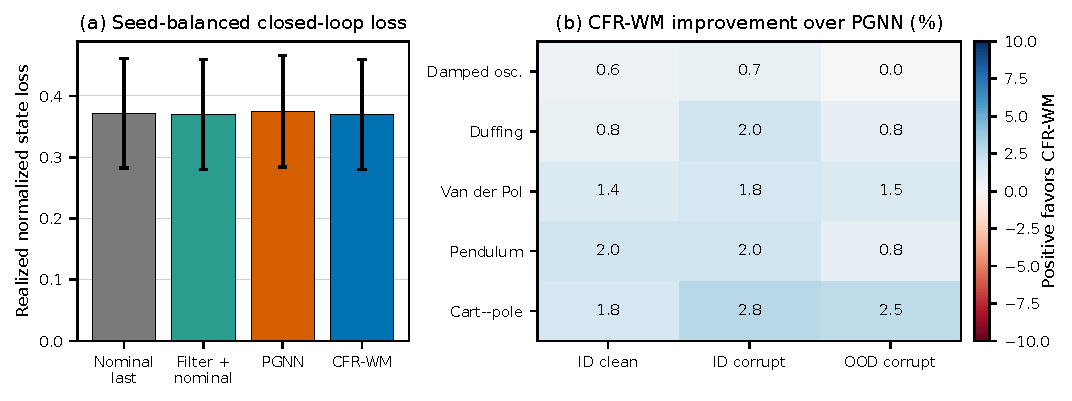
\includegraphics[width=0.94\textwidth]{figures/FigClosedLoop.pdf}
\caption{Closed-loop aggregate and heterogeneity. Error bars in (a) are SD
across eight seed-level aggregates; heat-map entries in (b) are seed means.}
\label{fig:supp-closed-loop}
\end{figure*}

\section{Measured-Flight Protocol and Full Results}

The external data set contains timestamped position, linear velocity, Euler
attitude, angular rates, and four motor commands. The reduced nominal prior
uses mass-normalized thrust, linear drag, an Euler-angle kinematic
approximation, inertia-scaled motor moments, and angular damping. The learned
residual retains the same 0.25 normalized bound used in the controlled
benchmark. Training uses only the designated training flight family;
development selects the learning rate from $\{10^{-3},3\times10^{-3}\}$ on a
separate seed. Five final seeds are then fit once. Sliding evaluation windows
do not cross flight boundaries.

Table~\ref{tab:supp-external-normalized} reports full-state NRMSE for every
method, context condition, and horizon. Table~\ref{tab:supp-external-physical}
gives position and velocity errors. The nominal prior has no training-seed
variation, so its reported SD is zero.

\begin{table*}[!t]
\centering
\caption{External full-state NRMSE, mean $\pm$ SD across training seeds after
equal weighting of the three held-out flights.}
\label{tab:supp-external-normalized}
\resizebox{\textwidth}{!}{\begin{tabular}{llrrrr}
\toprule
Context & Horizon & CFR-WM & Unfiltered & Recurrent & Nominal \\
\midrule
As recorded & 25 & $0.389 \pm 0.012$ & $0.376 \pm 0.010$ & $0.388 \pm 0.008$ & $0.488$ \\
As recorded & 50 & $0.530 \pm 0.016$ & $0.518 \pm 0.019$ & $0.519 \pm 0.006$ & $0.790$ \\
Noise & 25 & $0.393 \pm 0.012$ & $0.387 \pm 0.010$ & $0.398 \pm 0.008$ & $0.498$ \\
Noise & 50 & $0.532 \pm 0.017$ & $0.523 \pm 0.018$ & $0.527 \pm 0.006$ & $0.797$ \\
Missing & 25 & $0.397 \pm 0.011$ & $0.386 \pm 0.008$ & $0.395 \pm 0.005$ & $0.495$ \\
Missing & 50 & $0.537 \pm 0.014$ & $0.527 \pm 0.020$ & $0.526 \pm 0.007$ & $0.792$ \\
Noise + missing & 25 & $0.401 \pm 0.011$ & $0.397 \pm 0.008$ & $0.405 \pm 0.005$ & $0.506$ \\
Noise + missing & 50 & $0.540 \pm 0.014$ & $0.534 \pm 0.019$ & $0.533 \pm 0.006$ & $0.799$ \\
\bottomrule
\end{tabular}
}
\end{table*}

\begin{table*}[!t]
\centering
\caption{External position and velocity RMSE in physical units.}
\label{tab:supp-external-physical}
\resizebox{\textwidth}{!}{\begin{tabular}{lrrrr}
\toprule
& \multicolumn{2}{c}{Position RMSE (m)} & \multicolumn{2}{c}{Velocity RMSE (m/s)} \\
Context & CFR-WM & Unfiltered & CFR-WM & Unfiltered \\
\midrule
As recorded & $0.078 \pm 0.003$ & $0.083 \pm 0.010$ & $0.249 \pm 0.015$ & $0.233 \pm 0.009$ \\
Noise & $0.091 \pm 0.003$ & $0.115 \pm 0.007$ & $0.257 \pm 0.014$ & $0.258 \pm 0.007$ \\
Missing & $0.081 \pm 0.005$ & $0.095 \pm 0.022$ & $0.259 \pm 0.014$ & $0.243 \pm 0.009$ \\
Noise + missing & $0.094 \pm 0.004$ & $0.125 \pm 0.017$ & $0.267 \pm 0.014$ & $0.268 \pm 0.009$ \\
\bottomrule
\end{tabular}
}
\end{table*}

The probabilistic models use diagonal Gaussian marginals. The full external
uncertainty diagnostics are shown in Table~\ref{tab:supp-external-uncertainty}.

\begin{table*}[!t]
\centering
\caption{Measured-flight uncertainty diagnostics, averaged equally over held-
out flights and then over training seeds.}
\label{tab:supp-external-uncertainty}
\resizebox{\textwidth}{!}{\begin{tabular}{llrrrr}
\toprule
Condition & Method & NLL & Cov. & Width & Cal. error \\
\midrule
Recorded & CFR-WM & 2.264 & 0.608 & 0.453 & 0.178 \\
Recorded & Unfiltered residual & 0.794 & 0.716 & 0.526 & 0.099 \\
Noise & CFR-WM & 2.994 & 0.524 & 0.454 & 0.242 \\
Noise & Unfiltered residual & 2.361 & 0.565 & 0.528 & 0.217 \\
Missing & CFR-WM & 1.829 & 0.667 & 0.534 & 0.123 \\
Missing & Unfiltered residual & 0.735 & 0.779 & 0.685 & 0.053 \\
Combined & CFR-WM & 2.200 & 0.613 & 0.535 & 0.184 \\
Combined & Unfiltered residual & 1.130 & 0.703 & 0.688 & 0.124 \\
\bottomrule
\end{tabular}
}
\end{table*}

\begin{figure*}[!t]
\centering
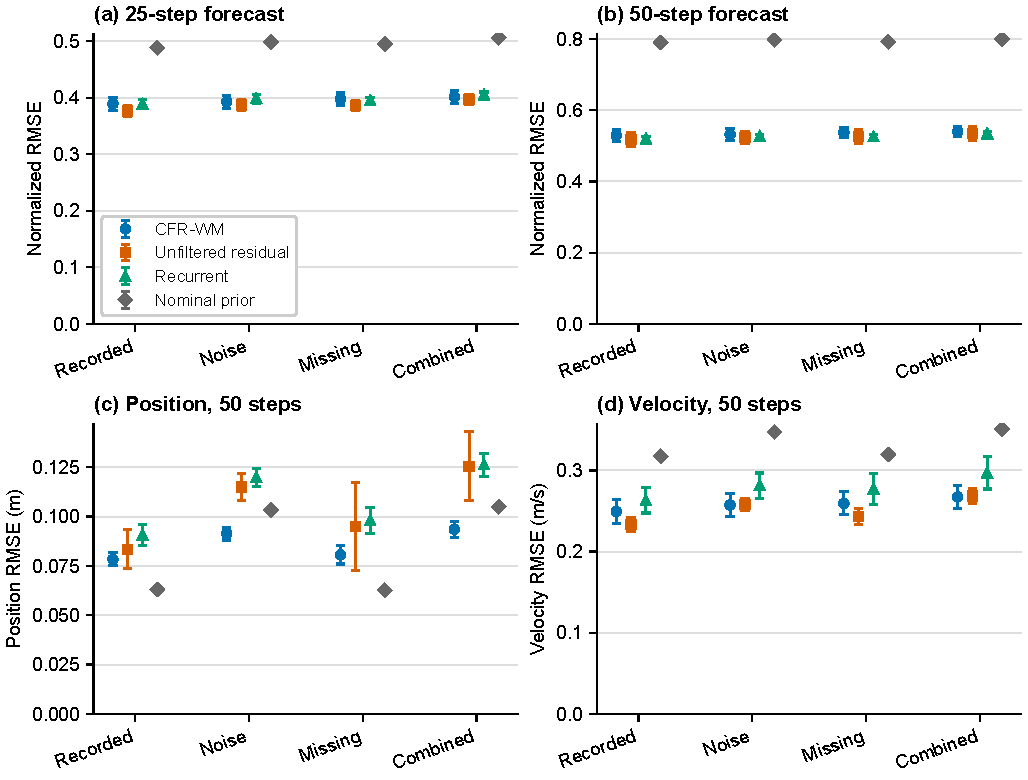
\includegraphics[width=0.94\textwidth]{figures/Fig4.pdf}
\caption{Measured-flight forecast errors by method, context condition, and
horizon. Position and full-state errors need not rank models identically.}
\label{fig:supp-external}
\end{figure*}


\end{document}
